%%%%%%%%%%%%%%%%%%%%%%%%%%%%%%%%%%%%%%%%
% University Assignment Title Page
% LaTeX Template
% Version 1.0 (27/12/12)
%
% This template has been downloaded from:
% http://www.LaTeXTemplates.com
%
% Original author:
% WikiBooks (http://en.wikibooks.org/wiki/LaTeX/Title_Creation)
%
% License:
% CC BY-NC-SA 3.0 (http://creativecommons.org/licenses/by-nc-sa/3.0/)
%
% Instructions for using this template:
% This title page is capable of being compiled as is. This is not useful for
% including it in another document. To do this, you have two options:
%
% 1) Copy/paste everything between \begin{document} and \end{document}
% starting at \begin{titlepage} and paste this into another LaTeX file where you
% want your title page.
% OR
% 2) Remove everything outside the \begin{titlepage} and \end{titlepage} and
% move this file to the same directory as the LaTeX file you wish to add it to.
% Then add \input{./title_page_1.tex} to your LaTeX file where you want your
% title page.
%
%%%%%%%%%%%%%%%%%%%%%%%%%%%%%%%%%%%%%%%%%
%\title{Title page with logo}
%----------------------------------------------------------------------------------------
%	PACKAGES AND OTHER DOCUMENT CONFIGURATIONS
%----------------------------------------------------------------------------------------

\documentclass[12pt]{article}
\usepackage[utf8]{inputenc}
\usepackage{amsmath}
\usepackage{graphicx}
\usepackage{lmodern}
\usepackage{hyperref}
\usepackage{tabularx}
\usepackage{amsmath}
\usepackage{float}
\usepackage[table]{xcolor}
\usepackage{booktabs}% http://ctan.org/pkg/booktabs

\usepackage{fancyhdr}

\newcommand{\tabitem}{~~\llap{\textbullet}~~}
\newcommand{\HRule}{\rule{\linewidth}{0.5mm}} % Defines a new command for the horizontal lines, change thickness here

\pagestyle{fancy}
\fancyhf{}
\rhead{Mission 1 -- Group G}
\lhead{\textit{LINGI2252}}
\cfoot{\thepage}

\begin{document}
    \begin{titlepage}
        \center % Center everything on the page

        %----------------------------------------------------------------------------------------
        %	HEADING SECTIONS
        %----------------------------------------------------------------------------------------

        \textsc{\LARGE Université Catholique de Louvain }\\[0.8cm] % Name of your university/college
        
\includegraphics[scale=0.45]{epl.jpg}
         \\[1.5cm]
        \textsc{\Large LINGI2252}\\[0.5cm] % Major heading such as course name
        \textsc{\large Software Maintenance and Evolution}\\[0.8cm] % Minor heading such as course title

        %----------------------------------------------------------------------------------------
        %	TITLE SECTION
        %----------------------------------------------------------------------------------------

        \HRule \\[0.4cm]
        { \huge \bfseries Mission 1: First prototype}\\[0.2cm] % Title of your document
        \HRule \\[1.5cm]

        %----------------------------------------------------------------------------------------
        %	AUTHOR SECTION
        %----------------------------------------------------------------------------------------

		\vfill
        \begin{minipage}{0.4\textwidth}
        \begin{flushleft} \large
        \emph{Authors:}\\
        \textbf{Group G}\\
        \textsc{Gustin}~Simon \\
        1171-14-00\\
        \textsc{Hallet}~Adrien \\
        3276-13-00\\
        \end{flushleft}
        \end{minipage}
        ~
        \begin{minipage}{0.4\textwidth}
        \begin{flushright} \large
        \emph{Professor:} \\
         \textsc{Mens}~Kim \\% Supervisor's Name
         \emph{Assistant:}\\
         \textsc{Duhoux}~Benoît
        \end{flushright}
        \end{minipage}\\[1cm]

        % If you don't want a supervisor, uncomment the two lines below and remove the section above
        %\Large \emph{Author:}\\
        %John~\textsc{Smith}\\[3cm] % Your name

        %----------------------------------------------------------------------------------------
        %	DATE SECTION
        %----------------------------------------------------------------------------------------

        {\large \today}\\[2cm] % Date, change the \today to a set date if you want to be precise

        %----------------------------------------------------------------------------------------
        %	LOGO SECTION
        %----------------------------------------------------------------------------------------

        % Include a department/university logo - this will require the graphicx package

        %----------------------------------------------------------------------------------------

        \vfill % Fill the rest of the page with whitespace
    \end{titlepage}

    \title{AAAAAA}
    \newpage

	\section{Introduction}
		For the course \textit{LINGI2252 -- Software Maintenance and Evolution}, we were asked to conceptualize and implement a (simulated) system for home automation and domotics.
		We already delivered a feature model, along with a lexicon and an example of usage scenario, provided here as well.
		
		In this document, we provide a new scenario, a (conceptual) class diagram of the code we implemented and a discussion of variablility points.
		
		The source code we implemented will be demonstrated later on in the year.
	
	\section{Lexicon}
		The following lexicon defines the meaning of words you can find in our feature model, class diagram and (to some extent) in our code.
		
		\begin{description}
            \item[Sensor] Physical device that measures the magnitude of real-life variables.
            \item[Light sensor] Sensor that measures the quantity of light in a room (lights being off or on).
            \item[Consumption sensor] Sensor that detects and records the consumption of different resources (power, water, etc).
            \item[Clock] Sensor that measures the time flying by (and can be used to set alarms at certain times).
            \item[Actuator] Physical device that is able to take actions in the physical world (make noise, light, move, etc).
            \item[Heavy appliance] Home systems that use lots of electricity (washing machine, dishwasher, oven, etc).
            \item[IoT] Internet of Things, the use of the internet for appliances like watches, clothes, ...
            \item[Hub] Physical and/or digital system to centralize a group of systems.
            \item[Connected device] Physical device that is (remotely) connected to the home automation system and that can thus be used as a sensor (for instance to measure how much energy the device consumes) or as an actuator (for example to turn it on or off).
        \end{description}
	
	\section{Scenarios}
		\subsection{First scenario}
			\textit{Note: this scenario is the one we provided with the first deliverable (for the previous lab).}
			
			It is time to fetch the kids at school and nobody else is available to bring them back. Your baby is in his bed and you have no choice but to leave him for a moment. You know it is a bad idea but hopefully you can rely on your \emph{Home Automation System}.

      		You leave home and set up the system via your smartphone.
      		Your \emph{smart door} locks itself up and redirects its \emph{intercom} feed to your smartphone since your door has a \emph{video sensor}. Because you also opted for a \emph{motion sensor} in the entrance, the \emph{anti-burglar} turns on and is ready to set the \emph{alarm} off, just in case.
      		On your smartphone, the \emph{audio sensor} in the baby's room calibrates itself to pick any irregularity up and acts as a \emph{babyphone}. The temperature in the baby's room will be kept constant thanks to the automatic heating system, so the baby is not too hot or too cold.
		
		\subsection{Second scenario}
			You come back late from work. You have had a rough day, you're stressed out and tired. You decide to relax, using your \emph{Home Automation System}.
			
			Once you are in your bedroom, you use your \emph{vocal command} and ask your house to close the \emph{curtains} and to turn on a dim \emph{light}. To get you in a better mood, you tell it to play some jazzy music (which it can do thanks to your \emph{connected radio}). You ask it as well to manage the \emph{temperature} in the room so that you feel more comfortable.
			
			After a while, you decide to take a bath. In order to not spend to much time in there, you ask your house to warn you once an hour has passed (which it can do thanks to a \emph{clock} and an \emph{alarm}).
			You can relax peacefully, knowing that your \emph{Home Automation System} will warn you if there is any danger such as a starting fire or a burglar entering in your house. You will not even have to get out of your bath to let your cat in the house.
			
			Isn't this great?
		
	\section{Feature model}		
        \begin{figure}[H]
            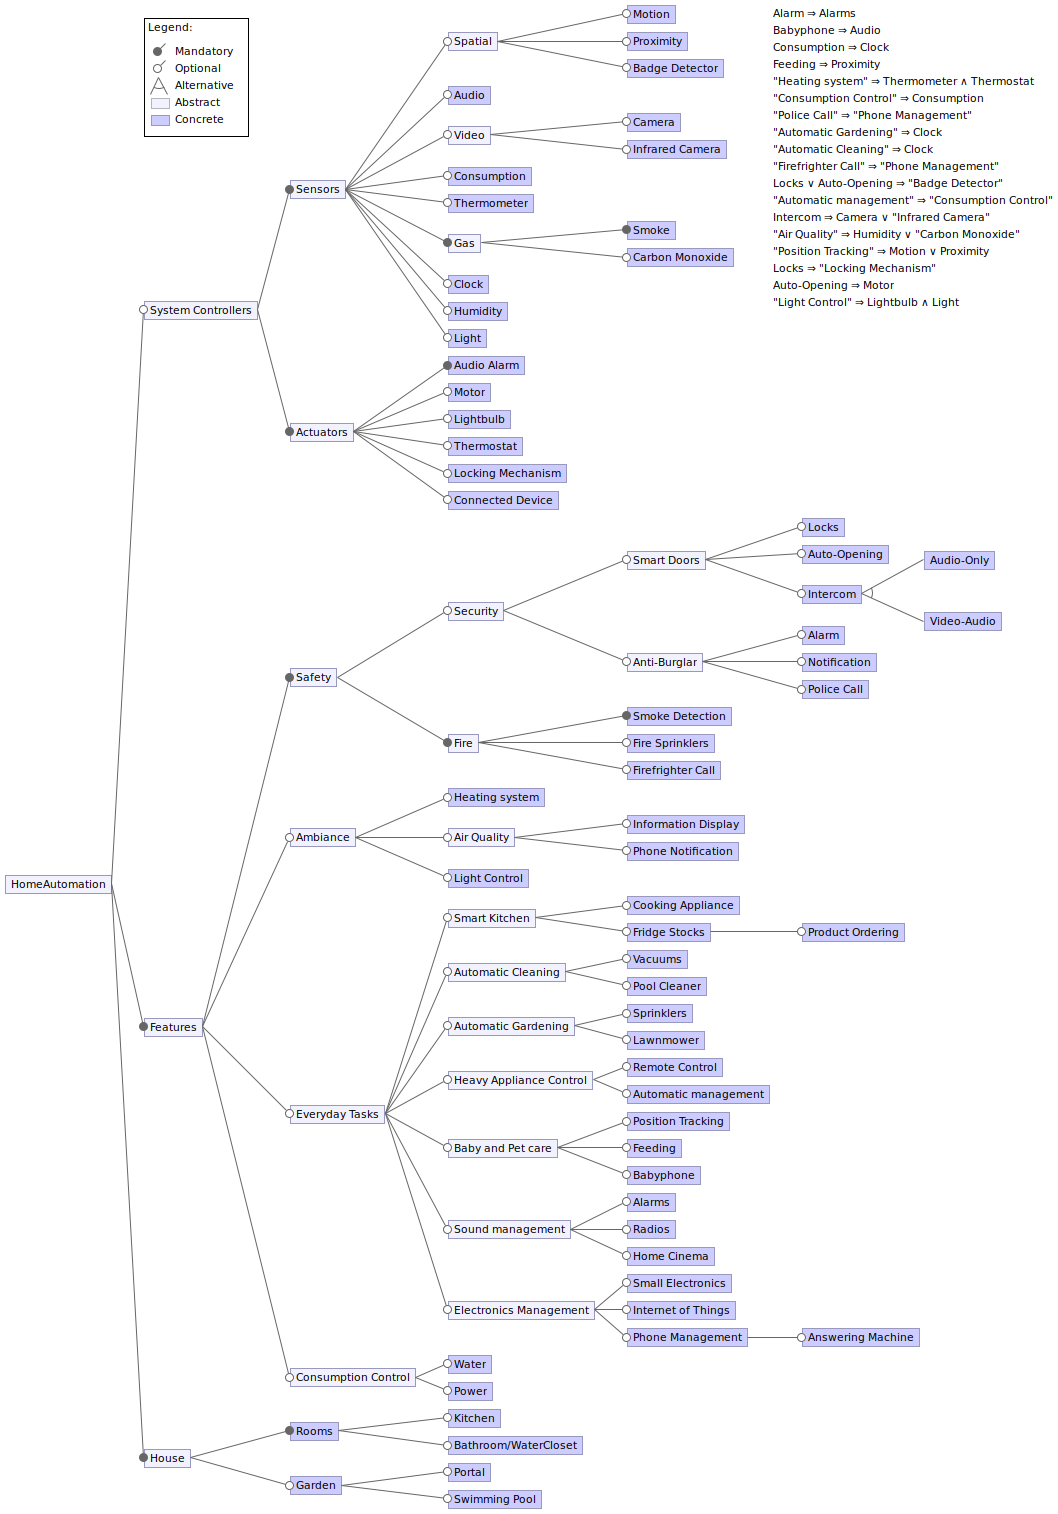
\includegraphics[width=0.9\textwidth]{FeatureModel_3.png}
        \end{figure}
	
	\section{Class diagram}
		This class diagram is highly conceptual (which means some internal methods and attributes, or even classes, may be missing). Nonetheless, it describes the general architecture of our code.
		
		\begin{figure}[H]
            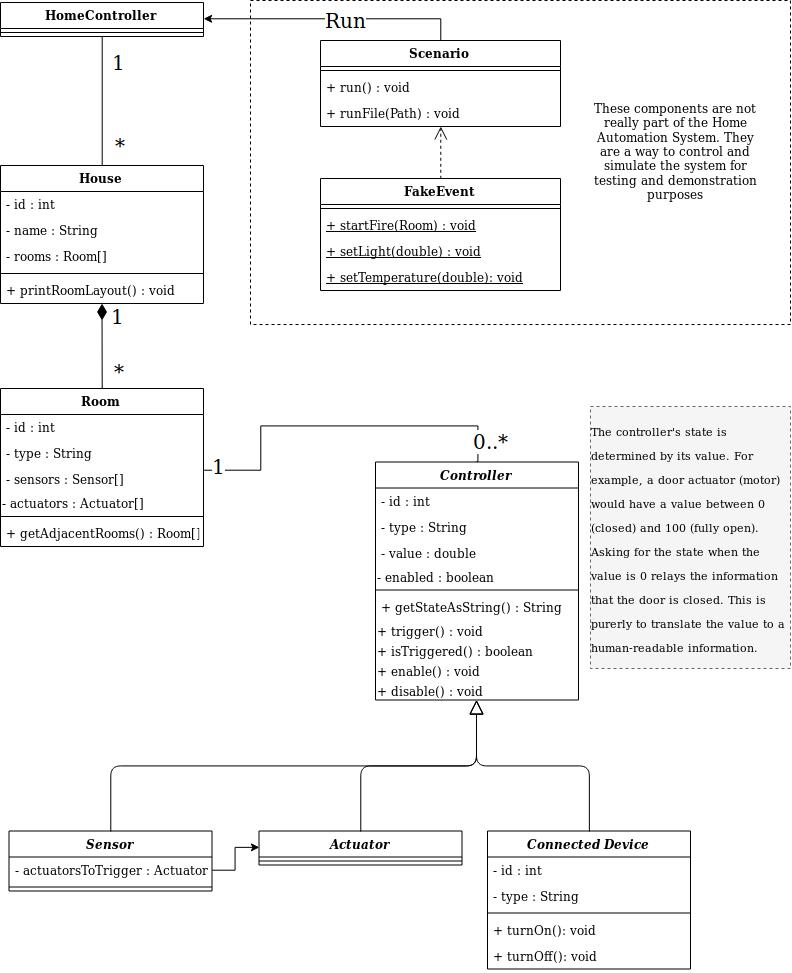
\includegraphics[width=0.9\textwidth]{class_diagram.png}
        \end{figure}
		
	\section{Potential variability points}
		As shown on the feature model, the only commonality we use is the smoke detector (along with an alarm) as it is the only one that is legally mandatory.
		
		In the current version of our code, we implemented several of the variability points shown on the same feature model. We chose them in order to be able to run several scenarios.
		Here is an exhaustive list of the features that we implemented and that can be used (or not) within different home configurations:
		\begin{itemize}
			\item TODO
		\end{itemize}
		
		In our code, we store the configuration of a house using a \textit{JSON} file.
	
	\section{Conclusion}
		In this document, we showed several documents that describe a home automation system.
		As we said, we implemented this system (which will be demonstrated later on during the semester).

\end{document}
